\chapter{Band Offset}
\label{chap:band-offset}

The next step on the bottom-up approach of the memristors is the simulation of the interfaces between the raw materials. Microscopy analysis shows the formation of Ti$_4$O$_7$ and Ti$_5$O$_9$ channels spanning a great part of TiO$_2$-based memristors (see Figure \ref{fig:canais-TiO}), but so far no theoretical work aiming to describe the electronic structure of such interface was presented. It is known that bulk Ti$_4$O$_7$ and Ti$_5$O$_9$ are metals in high temperatures \cite{Bartholomew1969}, but in the nanometric scale it may not be the case. As shown in the last chapter, these oxygen-deficient phases might donate electrons from the IB to the host material of the memristor, changing its properties. The knowledge of the electronic properties of the interfaces is then paramount to further investigate the memristor. With that goal in mind, we build a supercell which contains the Ti$_4$O$_7$-TiO$_2$ interface and obtain the valence band-offset of this system, thus, a common reference for all electronic levels is available and the band alignment is understood. 

This offset is a key quantity for many applications, such as heterojunction solar cells, where incoming photons create electron-hole pairs which in turn are separated due to the band offset, giving rise to electrical current \cite{Liu2013}. Another example is the separation of charge carriers in photocatalysis using the TiO$_2$-rutile and -anatase mixed-phase, which was elucidated by this type of calculations \cite{Scanlon2013}. In both cases the excitation of the electron from the valence band (VB) to the conduction band (CB) of one material and the migration of this electron to the CB of the other material due to the fact that its CB is lower in energy is the desired process, thus, the knowledge of the band offset is paramount.

In periodic calculations such as the ones performed in this step, the energies are given with respect to an arbitrary reference \cite{Ihm1979,Blochl1994}. This is a problem when one tries to compare energy levels of different structures, as is the case of the study of interfaces. The standard procedure in this case is the calculation of the average electrostatic potential, which is performed for the isolated materials and for bulk-like regions of a supercell containing the interface, and then the levels are shifted accordingly.

All results in this chapter were obtained by means of DFT calculations. The parameters used in the simulations are presented in appendix \ref{sec:app-calc}.

\section{Construction of the Ti$_4$O$_7$-TiO$_2$ interface}
\label{sec:interface}

One of the key points in the process of building an interface between two distinct materials is to match two of the three unit cell vectors of each compound in the interfacial region. Usually the individual unit cells are multiplied along the interfacial vectors' directions in order to impose the lowest strain on each phase, such that the deviation from the bulk electronic structure away from the interface is minimum. For the materials considered here, this is a very difficult task, owing to the fact that TiO$_2$ and Ti$_4$O$_7$ present very different unit cells (see sections \ref{sec:tio2} and \ref{sec:magneli} respectively).

To overcome this difficulty, two operations are performed to derive the Ti$_4$O$_7$ Magnéli structure from the TiO$_2$-rutile. The first operation is to transform the TiO$_2$ tetragonal unit cell into the Ti$_4$O$_7$ triclinic cell \cite{Wood1981} (see table \ref{tab:struct-relax-prb}):
\begin{equation}
 \begin{array}{cccc}
 \left[ \begin{array}{c} a_M^{(n)} \\ b_M^{(n)} \\ c_M^{(n)} \end{array} \right] & = & \left[ \begin{array}{ccc} -1 & 0 & 1 \\ 1 & -1 & 1 \\ 0 & 0 & 2n-1 \end{array} \right] & \left[ \begin{array}{c} a_r \\ b_r \\ c_r \end{array} \right],
 \end{array}
 \label{eq:transf}
\end{equation}
where $a_M^{(n)}, b_M^{(n)}$ and $c_M^{(n)}$ are the cell vectors of the Magnéli structure of index $n$. This operation only affects the unit cell, the ions are not displaced, thus the crystal after the use of equation \ref{eq:transf} is still TiO$_2$-rutile. The second operation involves the displacement of the ions according to the formula \cite{Andersson1960,Harada2010,Anderson19671393}
\begin{equation}
  (121) \frac{1}{2}[0\bar{1}1],
  \label{eq:displ}
\end{equation}
where $(121)$ refers to a crystallographic plane of the rutile unit cell, and $[0\bar{1}1]$ is a vector of the same structure. This operation can be understood by successive displacements of ions. All atoms above a $(121)$ plane which was shifted $n$ times along the $c$ vector of the rutile structure [see figures \ref{fig:tio2} (a) and \ref{fig:ti4o7-struct}] are shifted by $\nicefrac{1}{2}[0\bar{1}1]$. This process is repeated until all the possible planes within the unit cell were considered. Since this operation affects only the atomic positions, the unit cell is preserved in this step.

The transformations presented above result in identical unit cells, thus, no strain is present at the interface. For our calculations, we use $n = 4$ in equation \ref{eq:transf} in order to derive the Ti$_4$O$_7$ unit cell as well as the same value of $n$ for the periodic displacements given by equation \ref{eq:displ}. Next, both cells are extended in the $c$ direction by periodic repetition, resulting in the structures presented in figure \ref{fig:struct-interface} (a) and (b). The last step was simply to join the structures at the plane secant to the $c$ axis, which resulted in the structure presented in figure \ref{fig:struct-interface} (c). The extension of the unit cells before performing this joining operation is justified by the necessity to create a bulk-like region for each compound inside the final supercell.
\begin{center}
 \begin{figure}[ht!]
   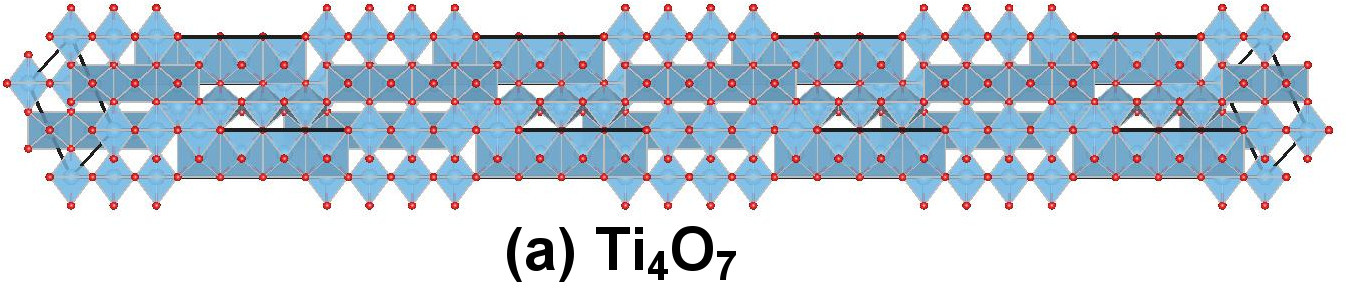
\includegraphics[width=0.5\textwidth]{img/ti4o7-big.jpg}
   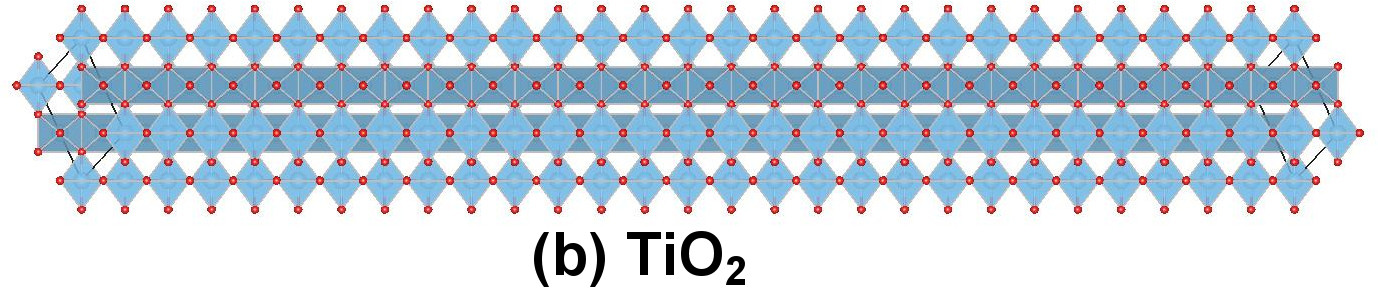
\includegraphics[width=0.5\textwidth]{img/tio2-big.jpg}
   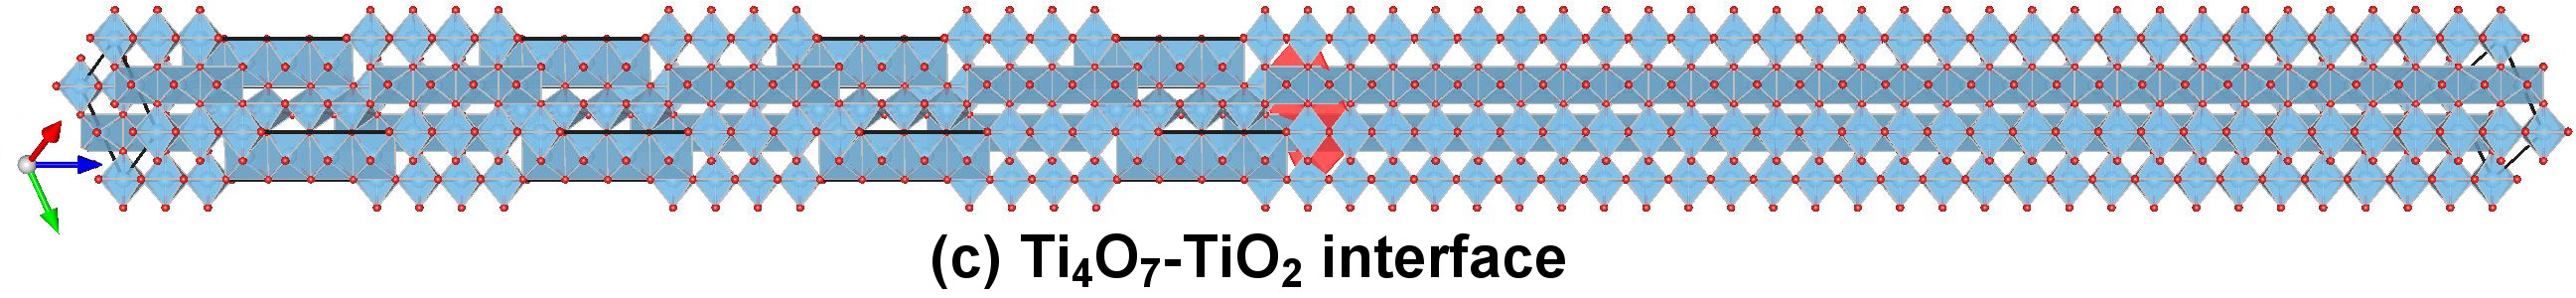
\includegraphics[width=1.0\textwidth]{img/interface-big.jpg}
  \caption{(a) Ti${}_4$O${}_7$ structure generated via the operations given by equations \ref{eq:transf} and \ref{eq:displ}, (b) TiO${}_2$ transformed according to equation \ref{eq:transf}, (c) and Ti${}_4$O${}_7$-TiO${}_2$ interface. The red plane in (c) indicates the interface region and the blue horizontal arrow corresponds to the $c$ crystal vector.}
  \label{fig:struct-interface}
 \end{figure}
\end{center}

\section{The band offset}
\label{sec:band-offset}

With the three structures obtained in the last section (both isolated materials and the supercell containing the interface), it is possible to calculate the valence band offset between the electronic levels of the bulk materials. The expression for the offset is given by \cite{Li2009b}
\begin{align}
 \Delta E_v(\text{TiO}_2|\text{Ti}_4\text{O}_7) =& \Delta E_{v,\phi}(\text{Ti}_4\text{O}_7)-\Delta E_{v,\phi}(\text{TiO}_2) \nonumber \\ &+\Delta E_{\phi}(\text{TiO}_2|\text{Ti}_4\text{O}_7),
 \label{eq:band-offset}
\end{align}
where $\Delta E_{v,\phi}(\text{Ti}_4\text{O}_7)$ and $\Delta E_{v,\phi}(\text{TiO}_2)$ are the differences between the Valence Band Maximum energy ($E_{VBM}$) and the electrostatic potential averaged over a certain volume of the unit cell of the isolated materials, while $\Delta E_{\phi}(\text{TiO}_2|\text{Ti}_4\text{O}_7)$ is the difference between the averaged electrostatic potential of the different materials calculated in bulk-like regions of the relaxed heterostructure supercell and the same averaged quantity obtained from the isolated material. An energy band diagram of the quantities involved in equation \ref{eq:band-offset} is presented in figure \ref{fig:bands-diagram}.
\begin{figure}[!ht]
\centering
  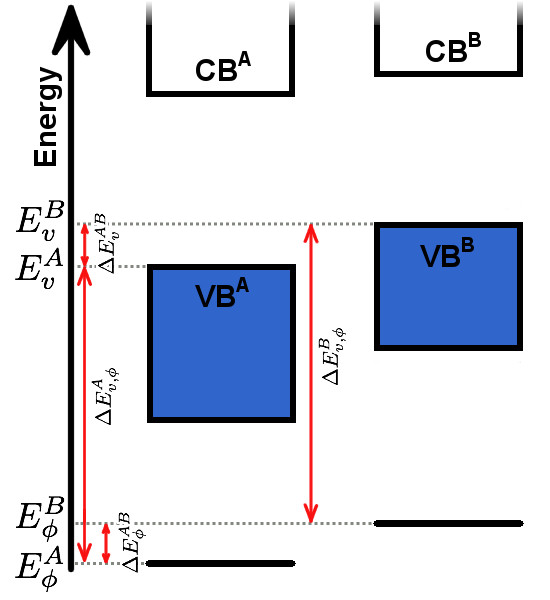
\includegraphics[width=0.5\textwidth]{img/band-offset-schematics.jpg}
  \caption{Band diagram of the valence band-offset between materials $A$ and $B$. $E_v^{A,B}$ and $E_{\phi}^{A,B}$ correspond to the energy of VBM and reference level of each material, respectively. $\Delta E_{v,\phi}^{A,B}$ is the energy difference between the reference energy level (in this work, the averaged electrostatic potential) and the VBM energy of compounds $A$ and $B$ respectively, while $\Delta E_{\phi}^{AB}$ and $\Delta E_v^{AB}$ are the offsets between the reference and the VBM's of the compounds.} 
  \label{fig:bands-diagram}
\end{figure}

Two of the quantities required by equation \ref{eq:band-offset} are readily obtained from DFT calculations using PBE$+U$ ($U = 5$ eV). This choice for the methodology is justified by the correct description of the oxygen-deficient phases presented in the previous chapter. In this manner, $E_{VBM}$ is obtained directly from the energy spectra of the isolated compounds, while the electrostatic potential [$\varphi(x,y,z)$] is obtained from the charge density calculated using the same method. The average of the potential along the $c$ axis is calculated by a simple integration along the planes secant to this vector,
\begin{equation}
 \phi(z) = \frac{1}{ab}\int_0^a \int_0^b \varphi(x,y,z) \, \mathrm{d}x \mathrm{d}y.
 \label{eq:partial}
\end{equation}
This average is plotted for all structures involved in the determination of the band offset in figure \ref{fig:potential}. In the potential profile it is possible to determine regions where the bulk potential is reproduced by the supercell results, being denoted by $\Delta z_1$ for the Ti$_4$O$_7$ part and $\Delta z_2$ for the TiO$_2$ part. The reference energy $E_{\phi}$ is obtained from the integration of $\phi(z)$ in those regions, either for the bulk materials as well as in the supercell. The values obtained from the bulk calculations for $E_{\phi}$ are used to calculate the first two terms of the right-hand side of equation \ref{eq:band-offset} while the ones obtained from the supercell are used in the last term.
\begin{center}
 \begin{figure}[ht!]
  \begin{center}
   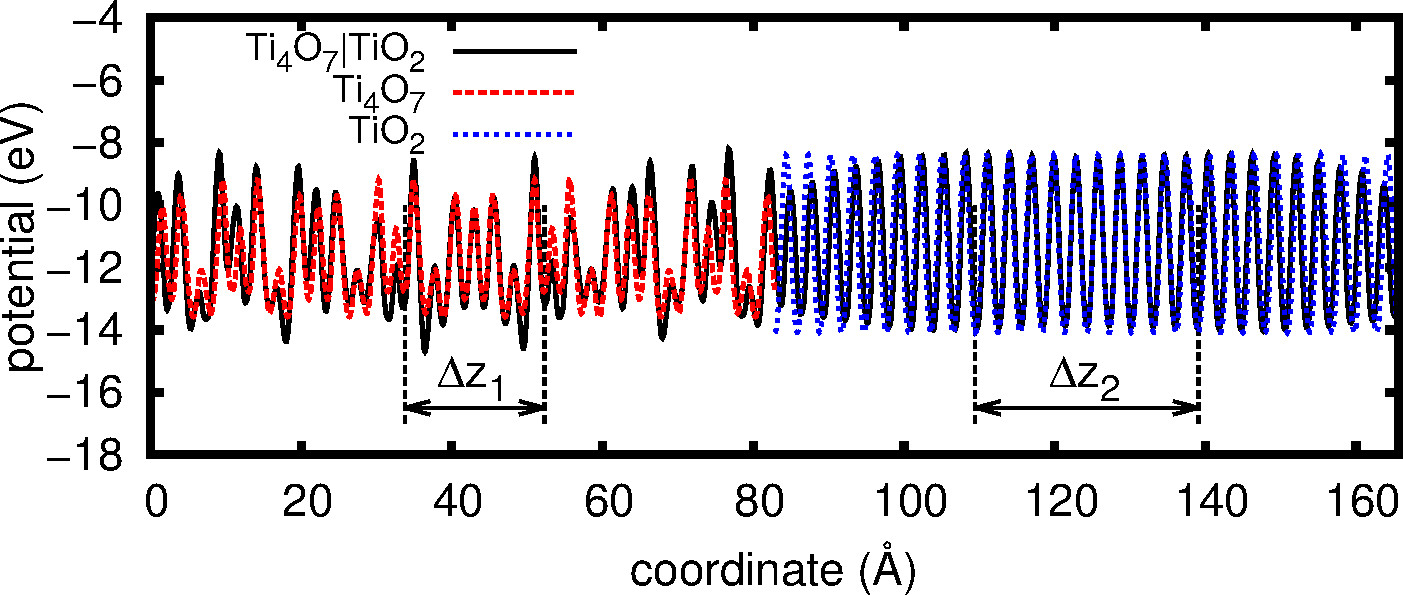
\includegraphics[width=0.9\columnwidth]{img/potential.jpg}
   \caption{Electrostatic potential profiles along the $c$ vector for all structures presented in this work: isolated TiO${}_2$ and Ti${}_4$O${}_7$, and the interface. $\Delta z_{1,2}$ denote the bulk-like region of the Ti$_4$O$_7$ and TiO$_2$ parts of the supercell, respectively.}
   \label{fig:potential} 
  \end{center}
 \end{figure}
\end{center}

The last step in this kind of calculation is the determination of the energy shift due to the strain introduced when interfacing the materials. Luckily in this case both cells used to build the interface are exactly the same by construction, thus, this final step presents no contribution. Finally, the calculated value for the valence band offset was $\Delta E_v (\text{TiO}_2|\text{Ti}_4\text{O}_7) = 2.18$ eV. The PDOS of both isolated systems is referenced by the TiO$_2$ VBM energy and the corresponding PDOS of Ti$_4$O$_7$ is shifted according to this result. These plots are presented in figure \ref{fig:pdos-bo}.

From the upper diagram in figure \ref{fig:pdos-bo} it is possible to extract two important informations: the localization of VBM and CBM in the compound system is at the Ti$_4$O$_7$ and TiO$_2$ respectively, and the energy difference between these levels---which is the bandgap---is 160 meV. However, by comparison with the results for the bulk Ti$_4$O$_7$ (section \ref{sec:magneli}) the last occupied level is the IB present in this structure, which can in turn donate electrons and $n$-dope the TiO$_2$. As the channels inside TiO$_2$-based memristors are made of Magnéli phases Ti$_4$O$_7$ and Ti$_5$O$_9$ channels immersed inside a TiO$_2$ matrix, this process of doping might take place inside the device, resulting in the change of the electronic properties of the active layer, and thus the electronic conductivity. This is further investigated in chapter \ref{chap:bandbend}, where the Poisson equation is solved for memristors and the role of the dopants in the transport properties is elucidated.

\begin{center}
 \begin{figure}[ht!]
  \begin{center}
   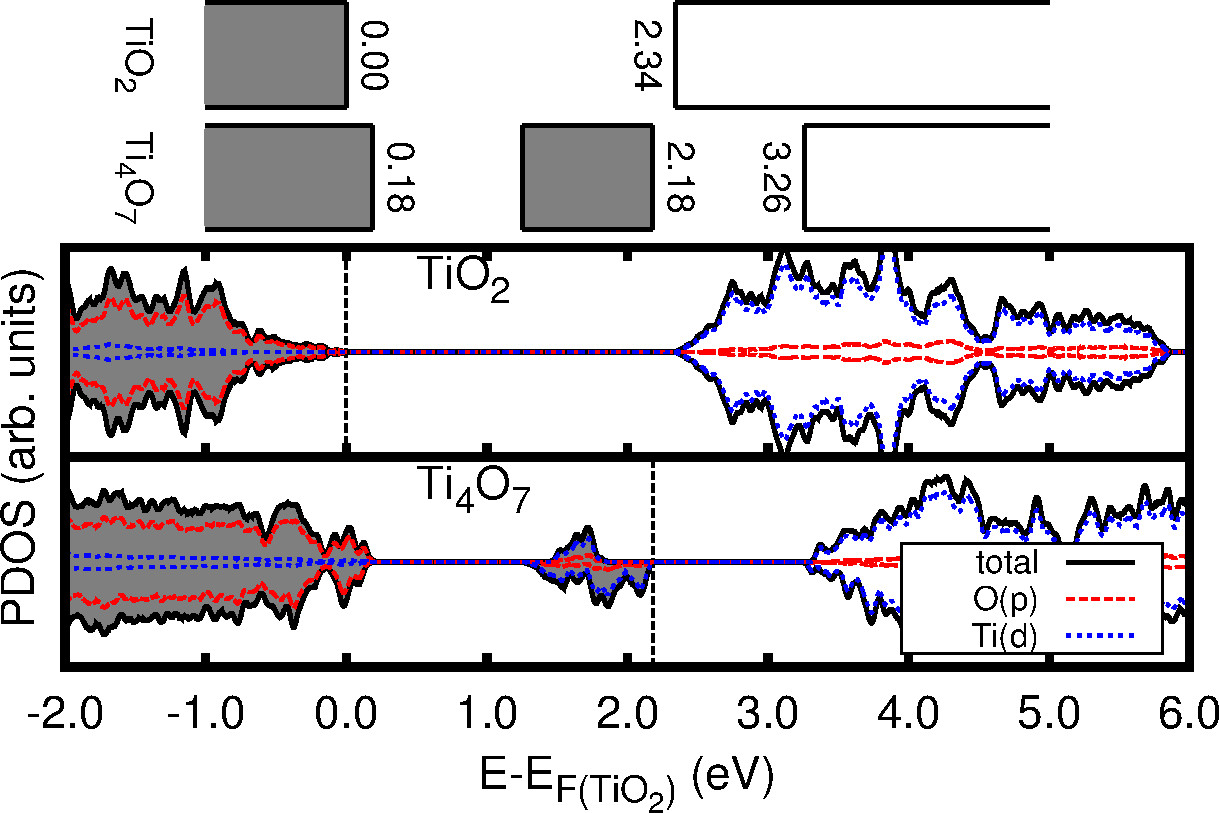
\includegraphics[width=0.8\columnwidth]{img/pdos-bo.jpg}
   \caption{PDOS of TiO${}_2$ rutile and Ti${}_4$O${}_7$. Gray shaded areas denote the occupied levels (below $E_F$, which is highlighted by the dotted vertical lines) and the two spin components are pictured by positive and negative values along the vertical axis. The upper panel shows the band alignment between the two materials.}
   \label{fig:pdos-bo} 
  \end{center}
 \end{figure}
\end{center}

Further evidence of the separation between VBM (more precisely, the Ti$_4$O$_7$ IB) and CBM by the interface is presented in the form of real-space projections of these frontier orbitals, given in figure \ref{fig:parchg-bo}. These projections are performed for the last occupied (VBM) and first unoccupied (CBM) electronic bands, using only the $\Gamma$ point eigenfunctions. From these projections it is possible to see that, while the VBM is mainly located on the Ti atoms of the Ti$_4$O$_7$ side which are close to the interface plane (presenting a small contribution of some Ti atoms of the TiO$_2$ structure), the CBM is delocalized over the same atomic species on the other side. As both levels present Ti(d) character, some degree of hybridization may be responsible for the contribution of the TiO$_2$ part to the VBM. The length of the $c$ vector also seemed to be of some influence in that result, as test calculations using a smaller supercell (the $c$ vector was half the size) present a higher degree of hybridization. Therefore, it is expected that in the limit of $c \rightarrow \infty$ the orbitals will be fully separated on the two phases.
\begin{center}
 \begin{figure}[ht!]
   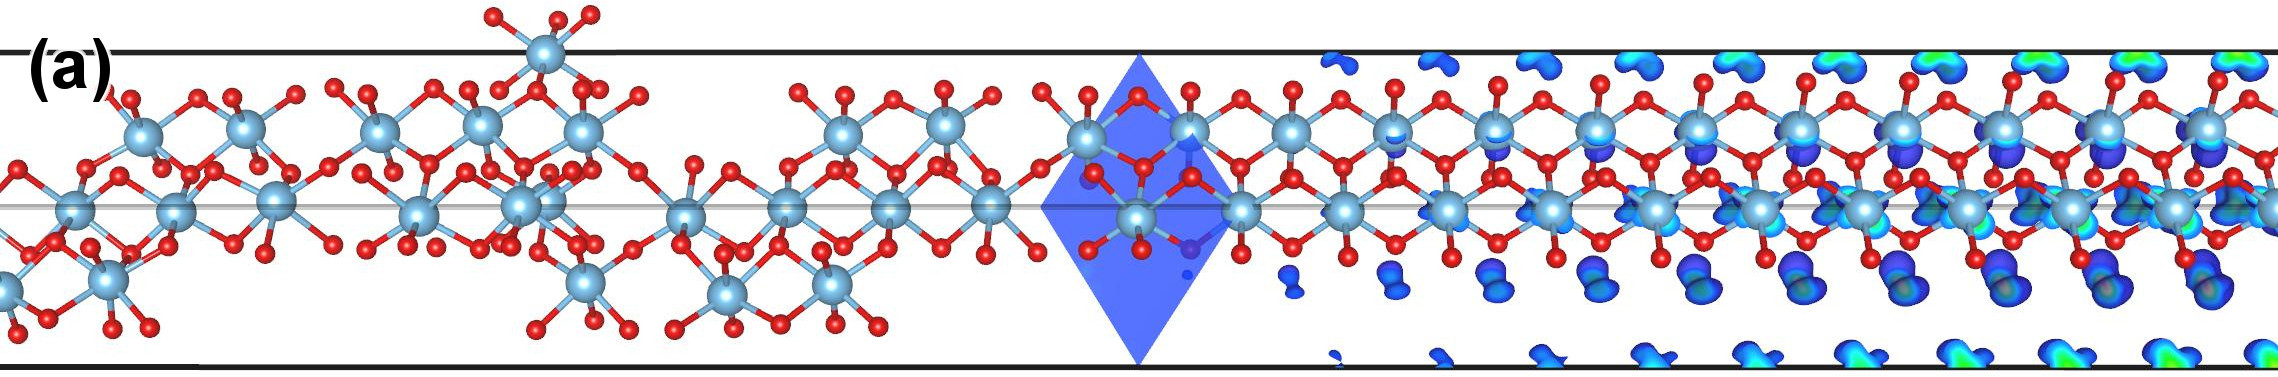
\includegraphics[width=\columnwidth]{img/parchg-cbm-gamma-ti4o7-tio2-new.jpg}
   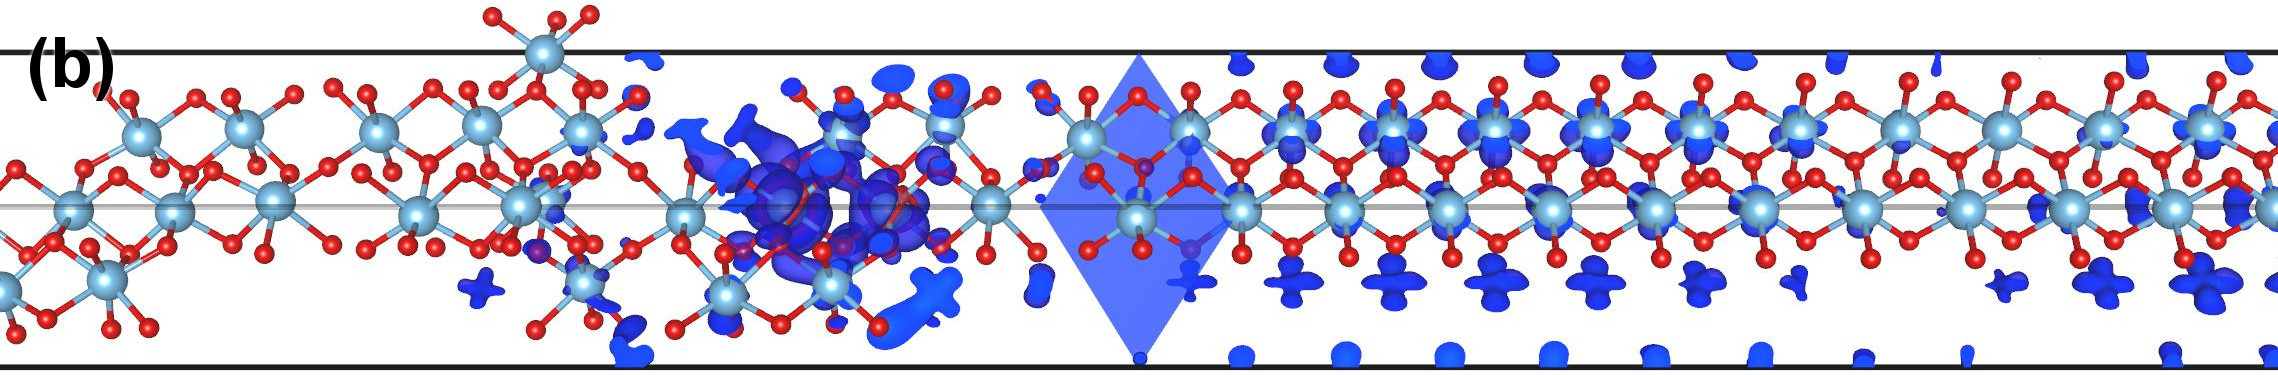
\includegraphics[width=\columnwidth]{img/parchg-vbm-gamma-ti4o7-tio2-new.jpg}
  \caption{Projected charge density for the (a) CBM and (b) VBM of the Ti${}_4$O${}_7$-TiO${}_2$ interface after ionic relaxation. The yellow plane features the interface region of the superstructure, being composed of Ti${}_4$O${}_7$ to the left and TiO${}_2$ to the right.}
  \label{fig:parchg-bo}
 \end{figure}
\end{center}

In conclusion, the results presented show that the IB lies inside the TiO$_2$ bandgap, close to the CM of this compound. This is type II band alignment, where the CB is in one material and the VB (in our case, it is the IB, which is the last occupied level) in the other. This suggests that electrons may be excited from Ti$_4$O$_7$ IB by means of an external perturbation, \textit{e. g.} an electric field of local heating in the active layer of the memristor, to the CB of the TiO$_2$ matrix, thus acting as dopants to this last material. This is a strong evidence of the role of the electronic processes in the memristive phenomena. It is important to emphasize that at this point no dynamical processes were considered: the band offset only is a static feature, but already capable of unraveling important aspects of the memristor that have never been probed before. All results presented in this section were published in Physical Review Applied \cite{Padilha2015}, and the article is attached in appendix \ref{sec:app-pub}.